\documentclass[journal abbreviation, manuscript]{copernicus}

\begin{document}

 %% \ SECTION 3
\section{Example model implementations}
- jupyter notebook for each example

\subsection{Methods}
%  quickly explain overview, explain methods for all of them shortly, with schematics, and put full system of equations & parameter tables in the Appendix!

\subsubsection{Model Structure: NPZD}

%%f
\begin{figure*}[t]
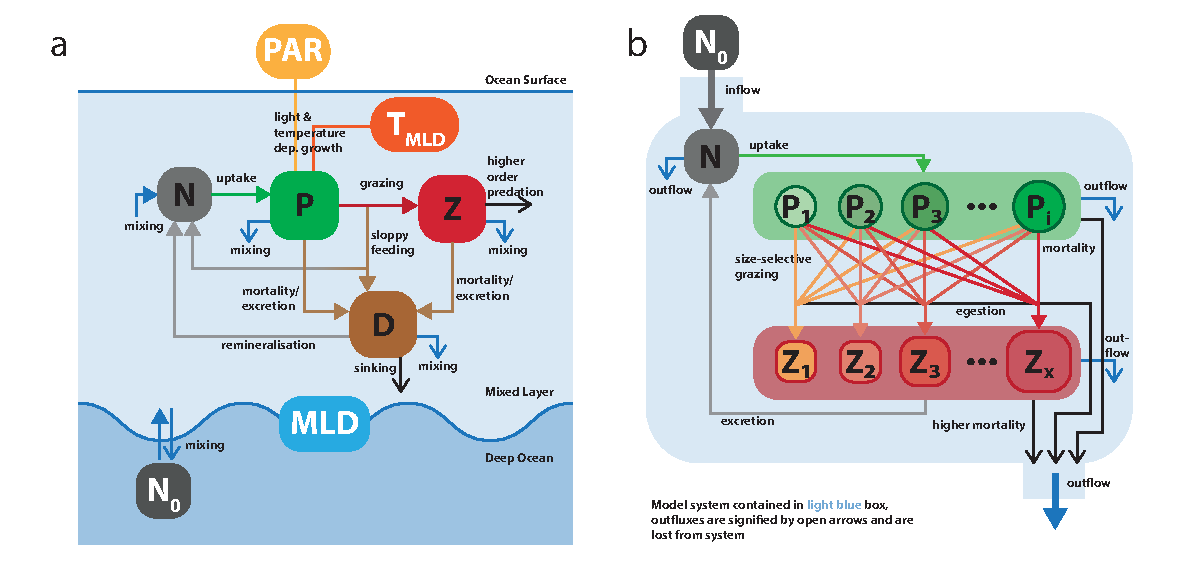
\includegraphics[width=15cm]{Figures/firstdraft_schematics/02__schematics_NPZDandChemostat.pdf}
\caption{TEXT}
\label{phydraschematics_1}
\end{figure*}

\subsubsection{Model Structure: Size-structured chemostat}

\subsubsection{Model Structure: Size-structured slab}
%%f
\begin{figure*}[t]
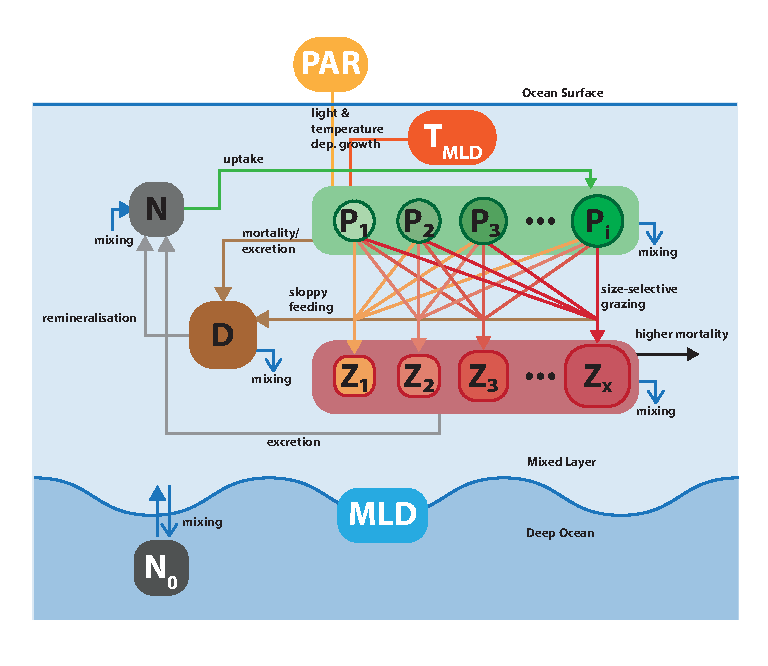
\includegraphics[width=12cm]{Figures/firstdraft_schematics/03__schematics_SizeStructSlab.pdf}
\caption{TEXT}
\label{phydraschematics_3}
\end{figure*}


% then move on to Results:
\subsection{Results}

\subsubsection{NPZD slab model}

%%f
\begin{figure}[t]
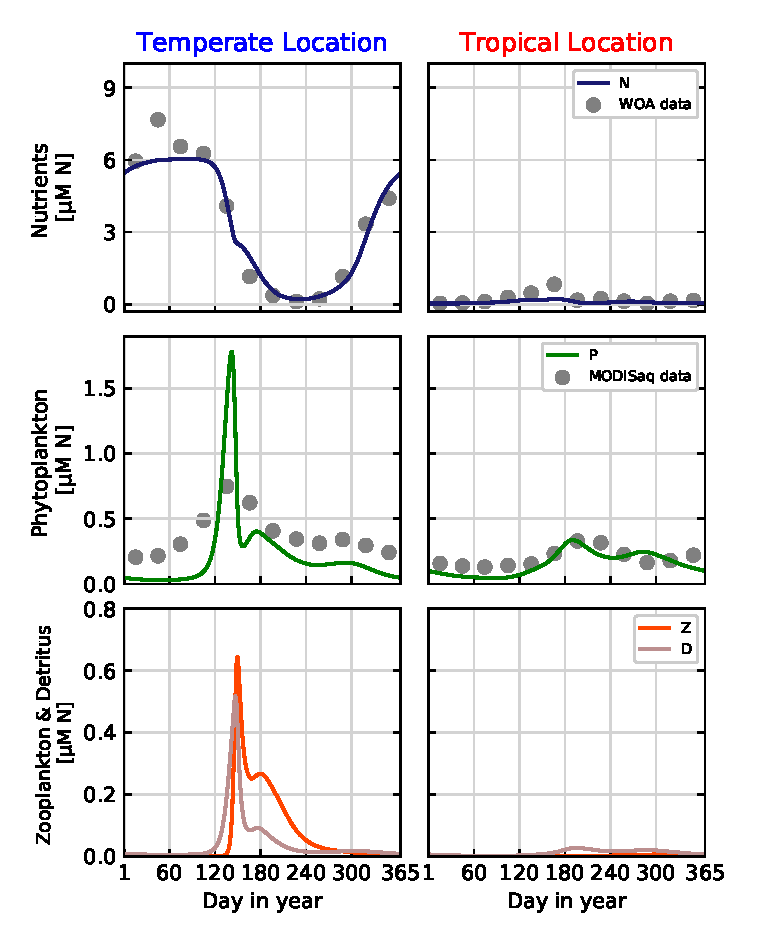
\includegraphics[width=8.3cm]{Figures/firstdraft_plots/02_NPZDslab.eps}
\caption{TEXT}
\end{figure}

\subsubsection{Size-structured NP40Z40 chemostat model}

\subsection{Size-structured NP20Z20D slab model}


\end{document}